% !TEX TS-program = pdflatex
% !TEX encoding = UTF-8 Unicode

\documentclass[12pt]{article}

\usepackage[utf8]{inputenc} 

\usepackage{geometry}
\geometry{a4paper} 
\geometry{margin=0.25in} 
\geometry{portrait}

\usepackage{amsmath}
\usepackage{physics}
\usepackage{tikz} 

\title{tikz figures}
\author{vijayabhaskar badireddi}

\begin{document}

\section*{Tikz figures}

\subsection*{figure 1}
\begin{center}

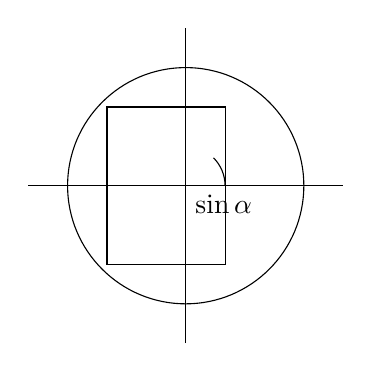
\begin{tikzpicture}[scale=0.5]
	\draw (0,0) node [anchor=north west] {$\sin\alpha$};
	\draw (-4,0) -- (4,0);
	\draw (0,-4) -- (0,4);
	\draw (0,0) circle [radius=3];
	\draw (1,2) rectangle (-2,-2);
	\draw (1,0) arc [start angle=0, end angle=45, radius=1];
\end{tikzpicture}
\end{center}

\subsection*{figure 2}

\begin{center}
\begin{tikzpicture}[scale=1]
	\draw (0,0) node [anchor=north west] {$O$};
	\draw [<->] (-5,0) -- (5,0);
	\draw [very thick,gray] (-4,0) -- (4,0);
	\draw [->] (0,-1) -- (0,4);
	\draw [very thin] (3,0) -- (0,3);
	\draw [-{latex},very thick] (0,3) -- ++(0.5,0.5);
	\draw (0.5,3.5) node [anchor=west] {$\dd\vec{B}$};
	\draw (3,0) node [anchor=north ] {$A(x,0)$};
	\draw (0,3) node [anchor=east] {$P(0,d)$};
	\draw (0,2.5) arc [start angle=270, end angle = 315,radius=0.5] ;
	\draw (0,2.5) node [anchor=north west] {$\theta$} ;
	\draw [very thick, red] (3,0) -- (3.1,0) ;
\end{tikzpicture}

\end{center}

\end{document}
